\section{Block Level Description}

\subsection{SPI/PSRBR}

\subsection{16-bit Kogge-Stone Adder}
The Kogge-Stone adder consists of four simple blocks connected in a complex way.

\noindent \todo{Lägg till bild på hur blocken sitter ihop.}

\subsubsection{Red}

\begin{table}[H]
  \caption{Logic table of red block.}
  \centering
  \begin{tabular}{cc|cc}
    \toprule
    $A_i$ & $B_i$ & $P$ & $G$ \\
    \midrule
    0 & 0 & 0 & 0 \\
    0 & 1 & 1 & 0 \\
    1 & 0 & 1 & 0 \\
    1 & 1 & 0 & 1 \\
    \bottomrule
    \label{tab:red}
  \end{tabular}
\end{table}

\begin{figure}[H]
  \centering
  \captionsetup{justification=centering}
  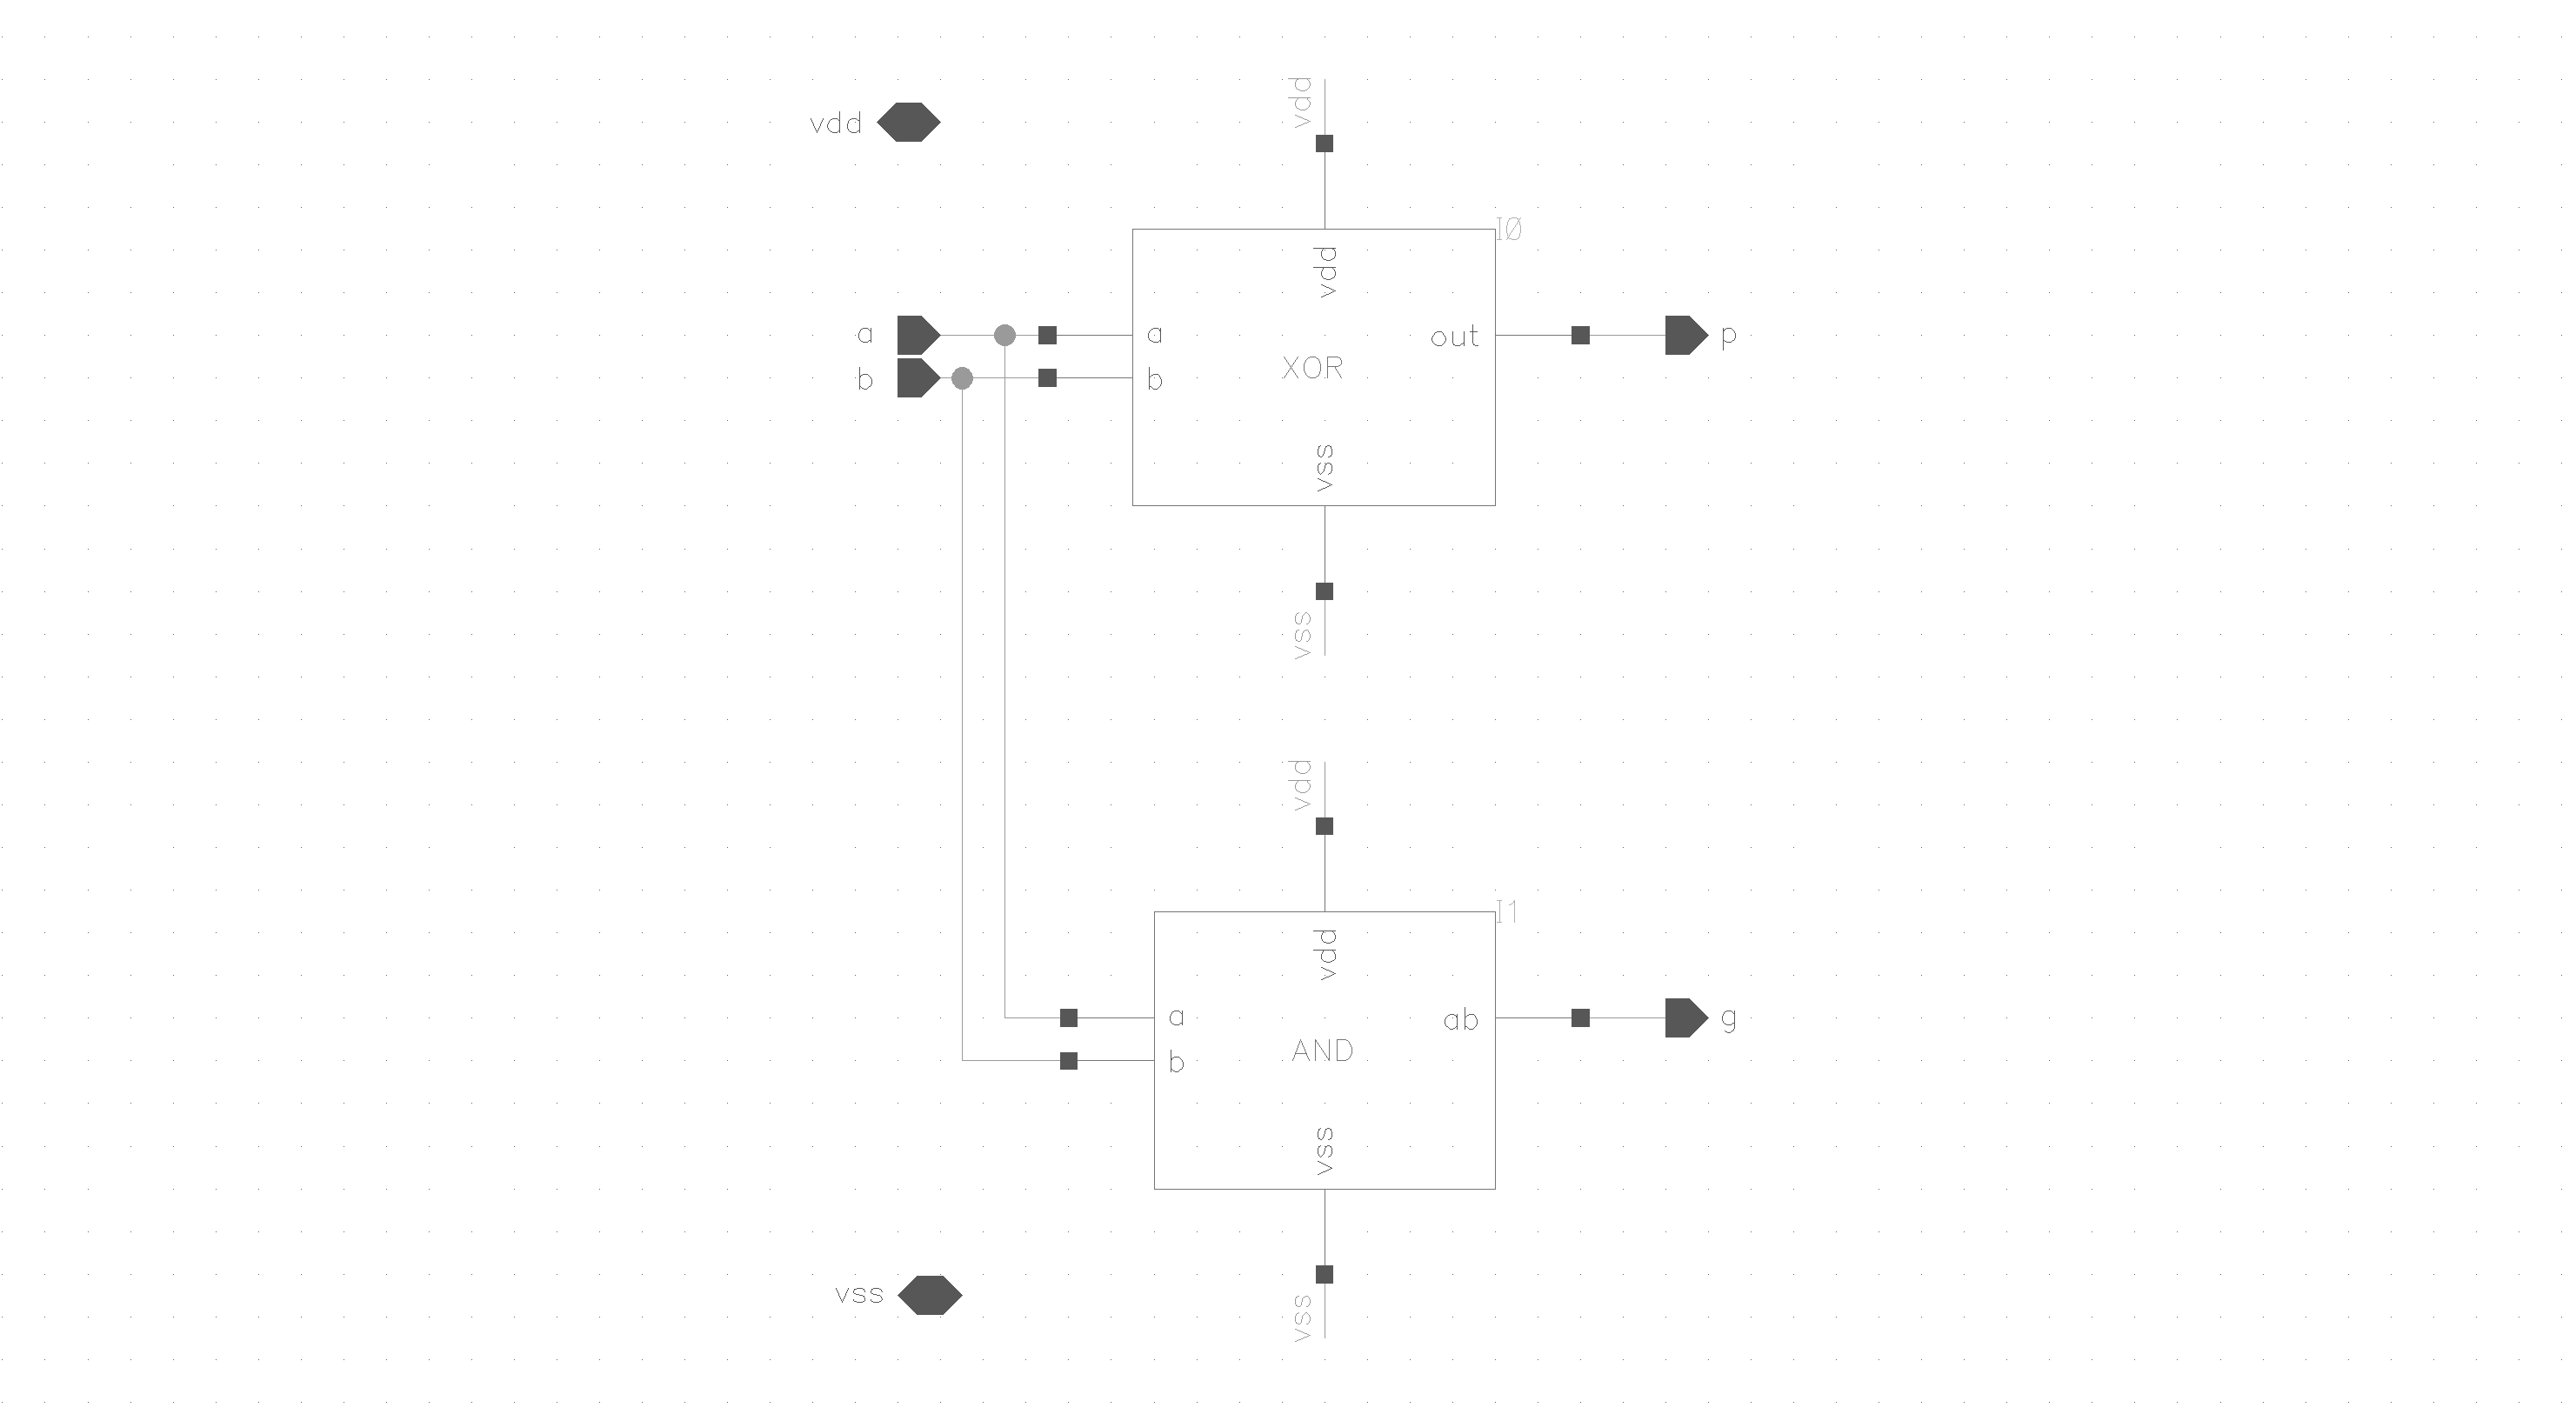
\includegraphics[clip,width=1.0\textwidth]{../figures/red}
  \caption{Figure shows whats inside the red block in the adder} \label{fig:red}
\end{figure}
\subsection{Comparator}

\subsubsection{Yellow}

\begin{table}[H]
  \caption{Logic table of yellow block.}
  \centering
  \begin{tabular}{cccc}
    \toprule
    Input & Function1 & Function2 & Output \\
    \midrule
    00 & 1 & 0& 1\\
    01 & 0 & 0 & 1\\
    10 & 0 & 0 & 1\\
    11 & 1 & 0 & 1\\
    \bottomrule
    \label{tab:yellow}
  \end{tabular}
\end{table}

\begin{figure}[H]
  \centering
  \captionsetup{justification=centering}
  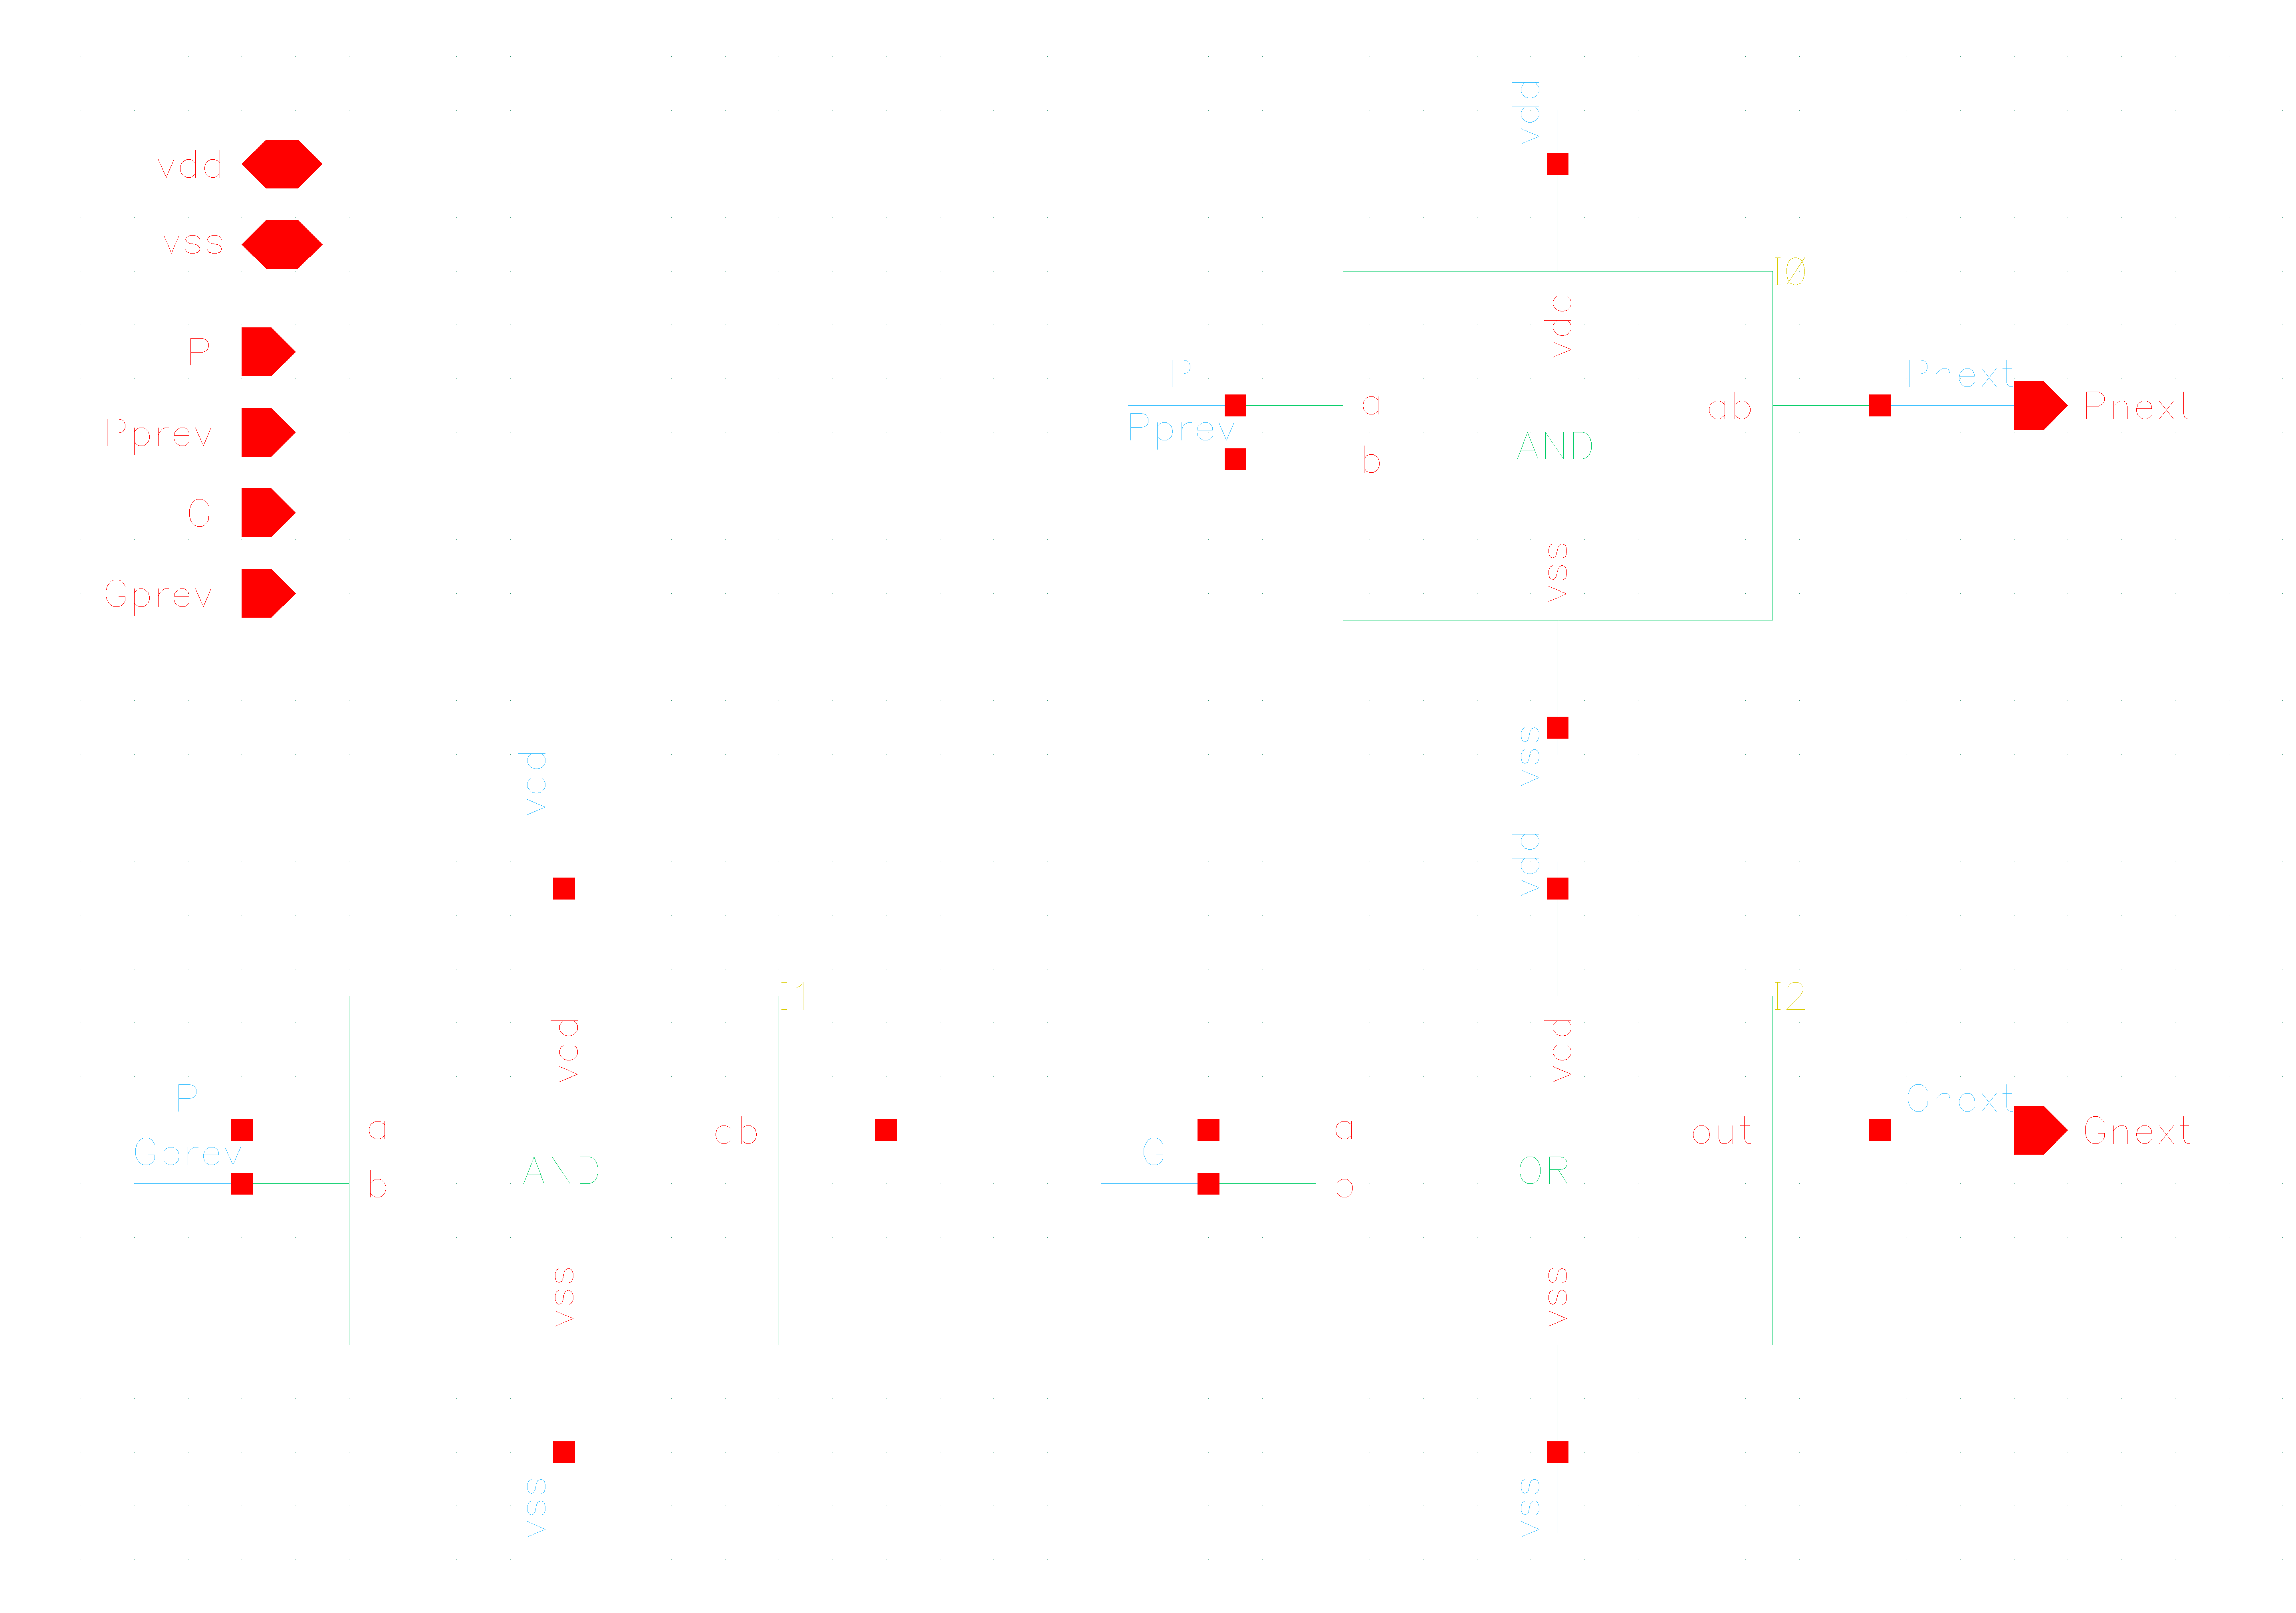
\includegraphics[clip,width=1.0\textwidth]{../figures/yellow}
  \caption{Figure shows whats inside the yellow block in the adder} \label{fig:yellow}
\end{figure}

\subsubsection{Yellow with carry}

\begin{table}[H]
  \caption{Logic table of yellow with carry block.}
  \centering
  \begin{tabular}{cccc}
    \toprule
    Input & Function1 & Function2 & Output \\
    \midrule
    00 & 1 & 0& 1\\
    01 & 0 & 0 & 1\\
    10 & 0 & 0 & 1\\
    11 & 1 & 0 & 1\\
    \bottomrule
    \label{tab:yellowcarry}
  \end{tabular}
\end{table}

\begin{figure}[H]
  \centering
  \captionsetup{justification=centering}
  \adjustbox{trim={0\width} {0\height} {0\width} {.4\height},clip}
  {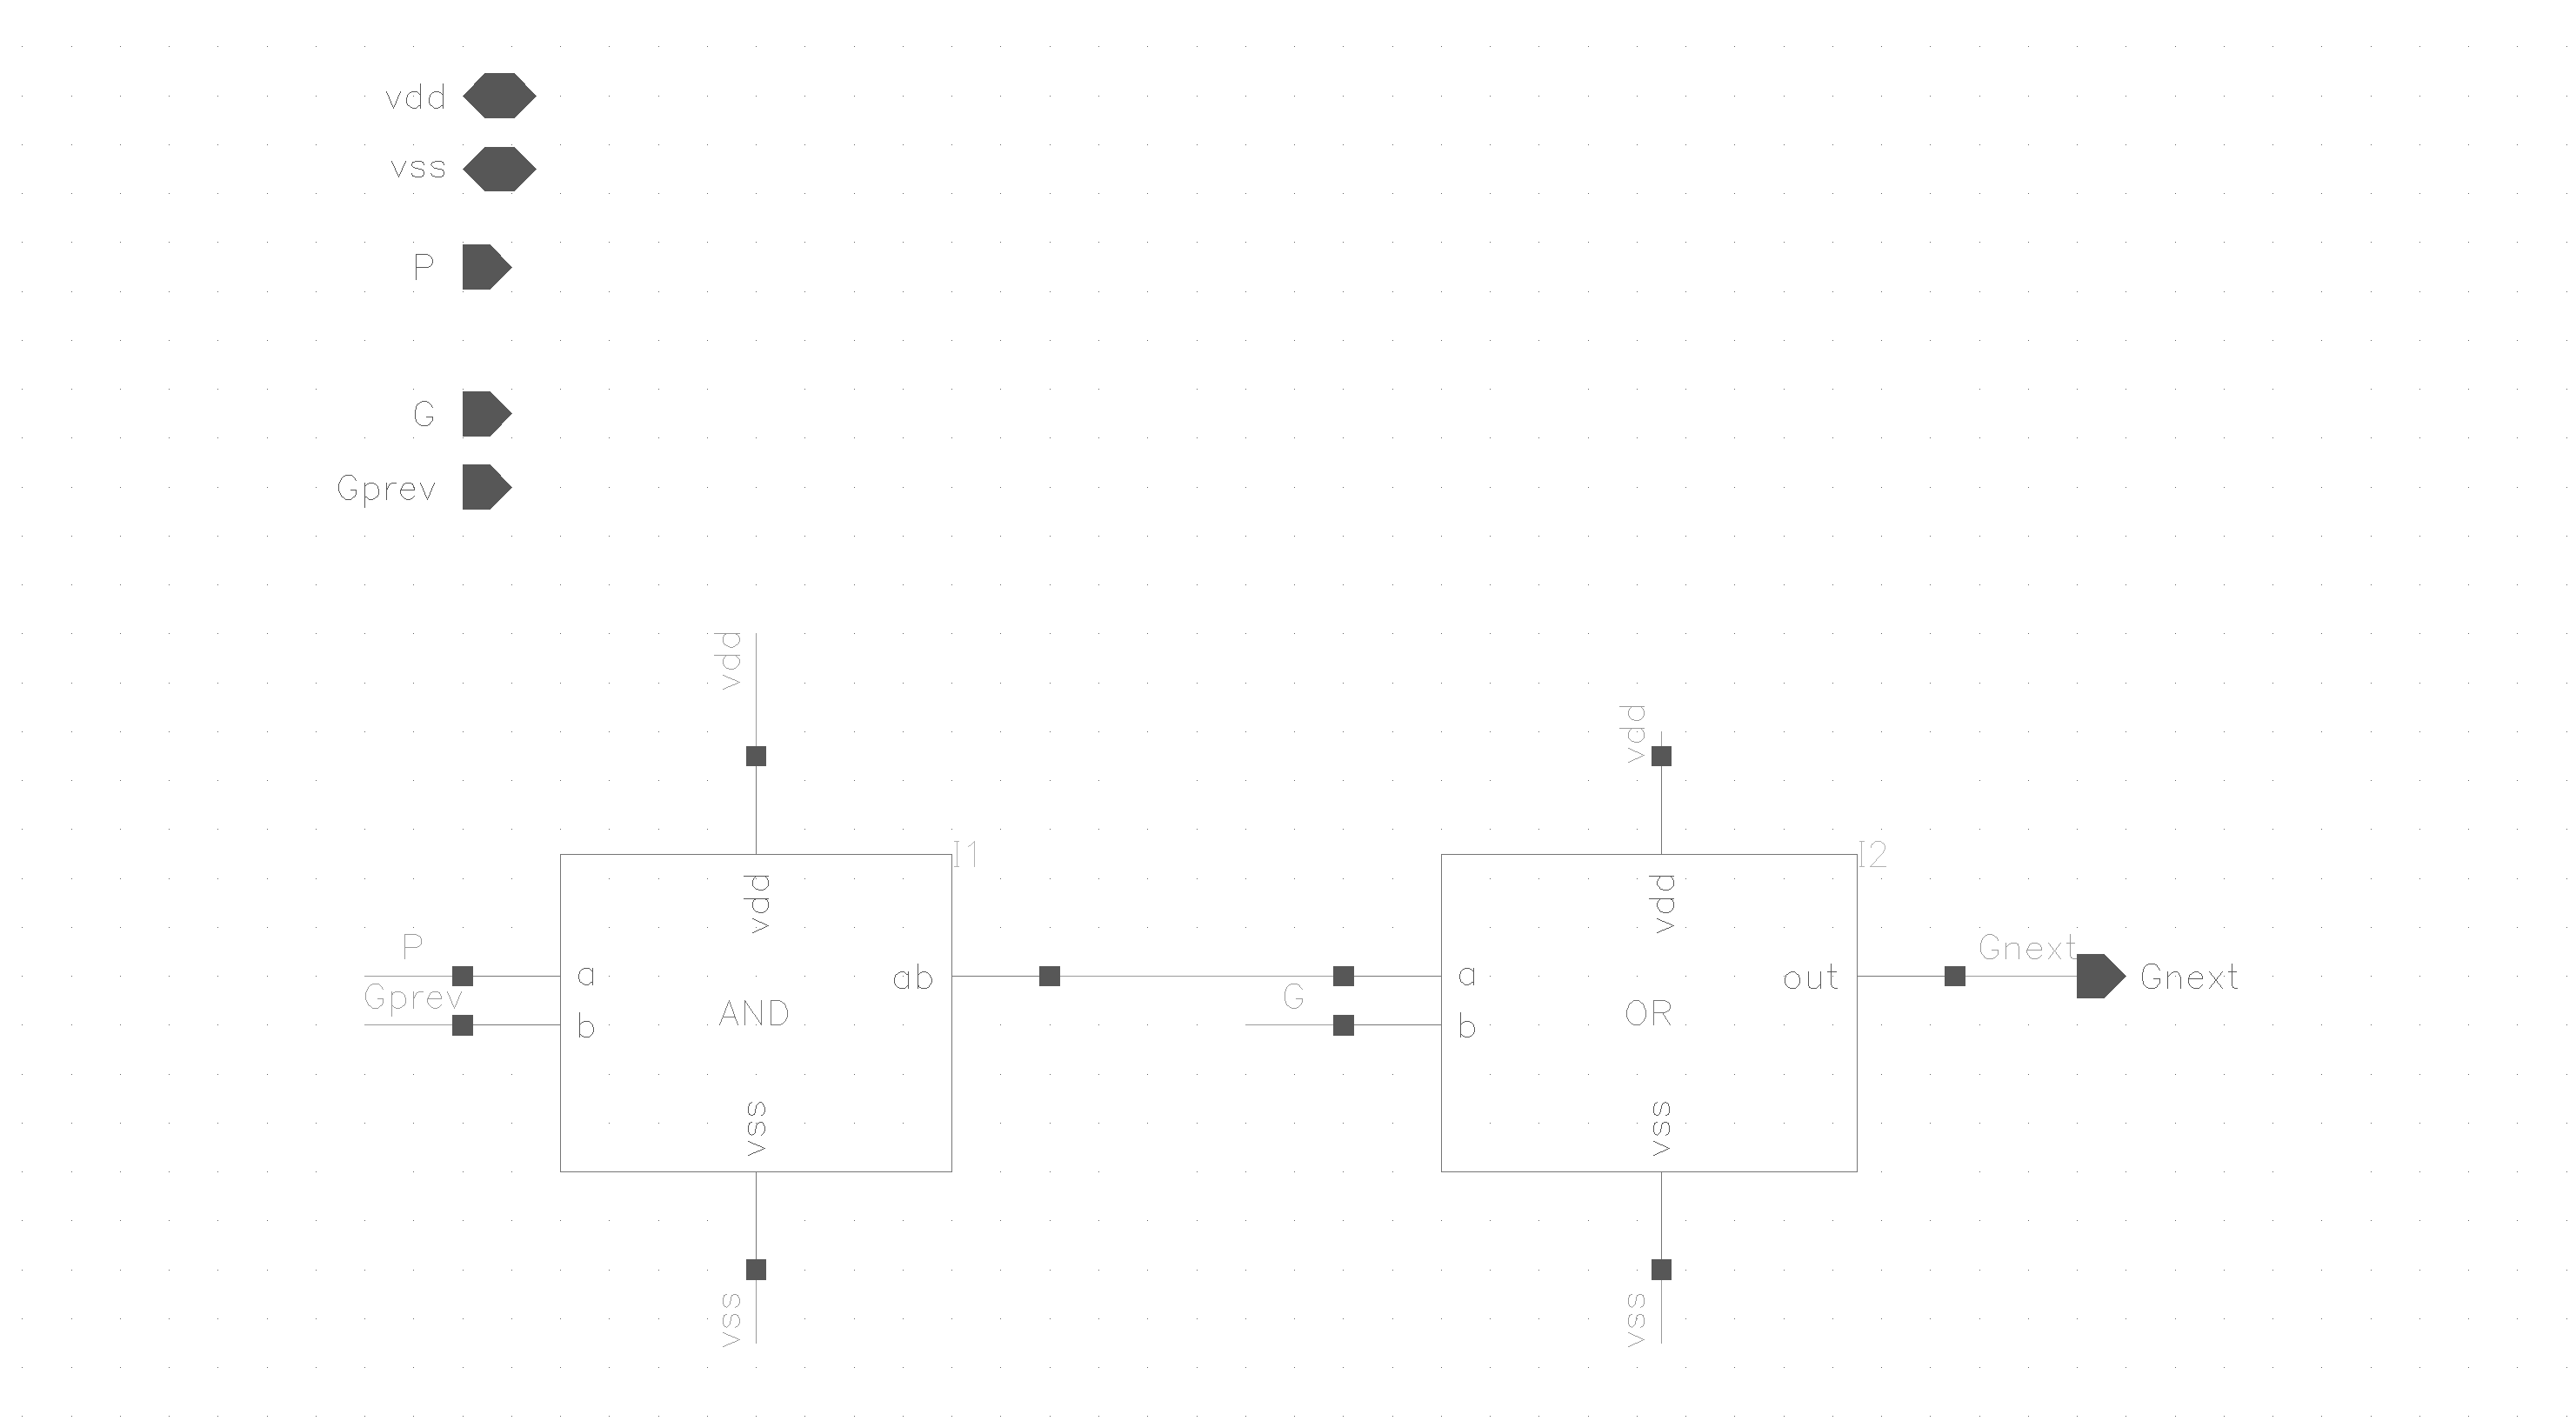
\includegraphics[width=1.0\textwidth]{../figures/yellow_carry}}
  \caption{Figure shows whats inside the yellow carry block in the adder} \label{fig:yellow_c}
\end{figure}

\subsubsection{Sum}

\begin{table}[H]
  \caption{Logic table of sum block.}
  \centering
  \begin{tabular}{cccc}
    \toprule
    Input & Function1 & Function2 & Output \\
    \midrule
    00 & 1 & 0& 1\\
    01 & 0 & 0 & 1\\
    10 & 0 & 0 & 1\\
    11 & 1 & 0 & 1\\
    \bottomrule
    \label{tab:sum}
  \end{tabular}
\end{table}

\begin{figure}[H]
  \centering
  \captionsetup{justification=centering}
  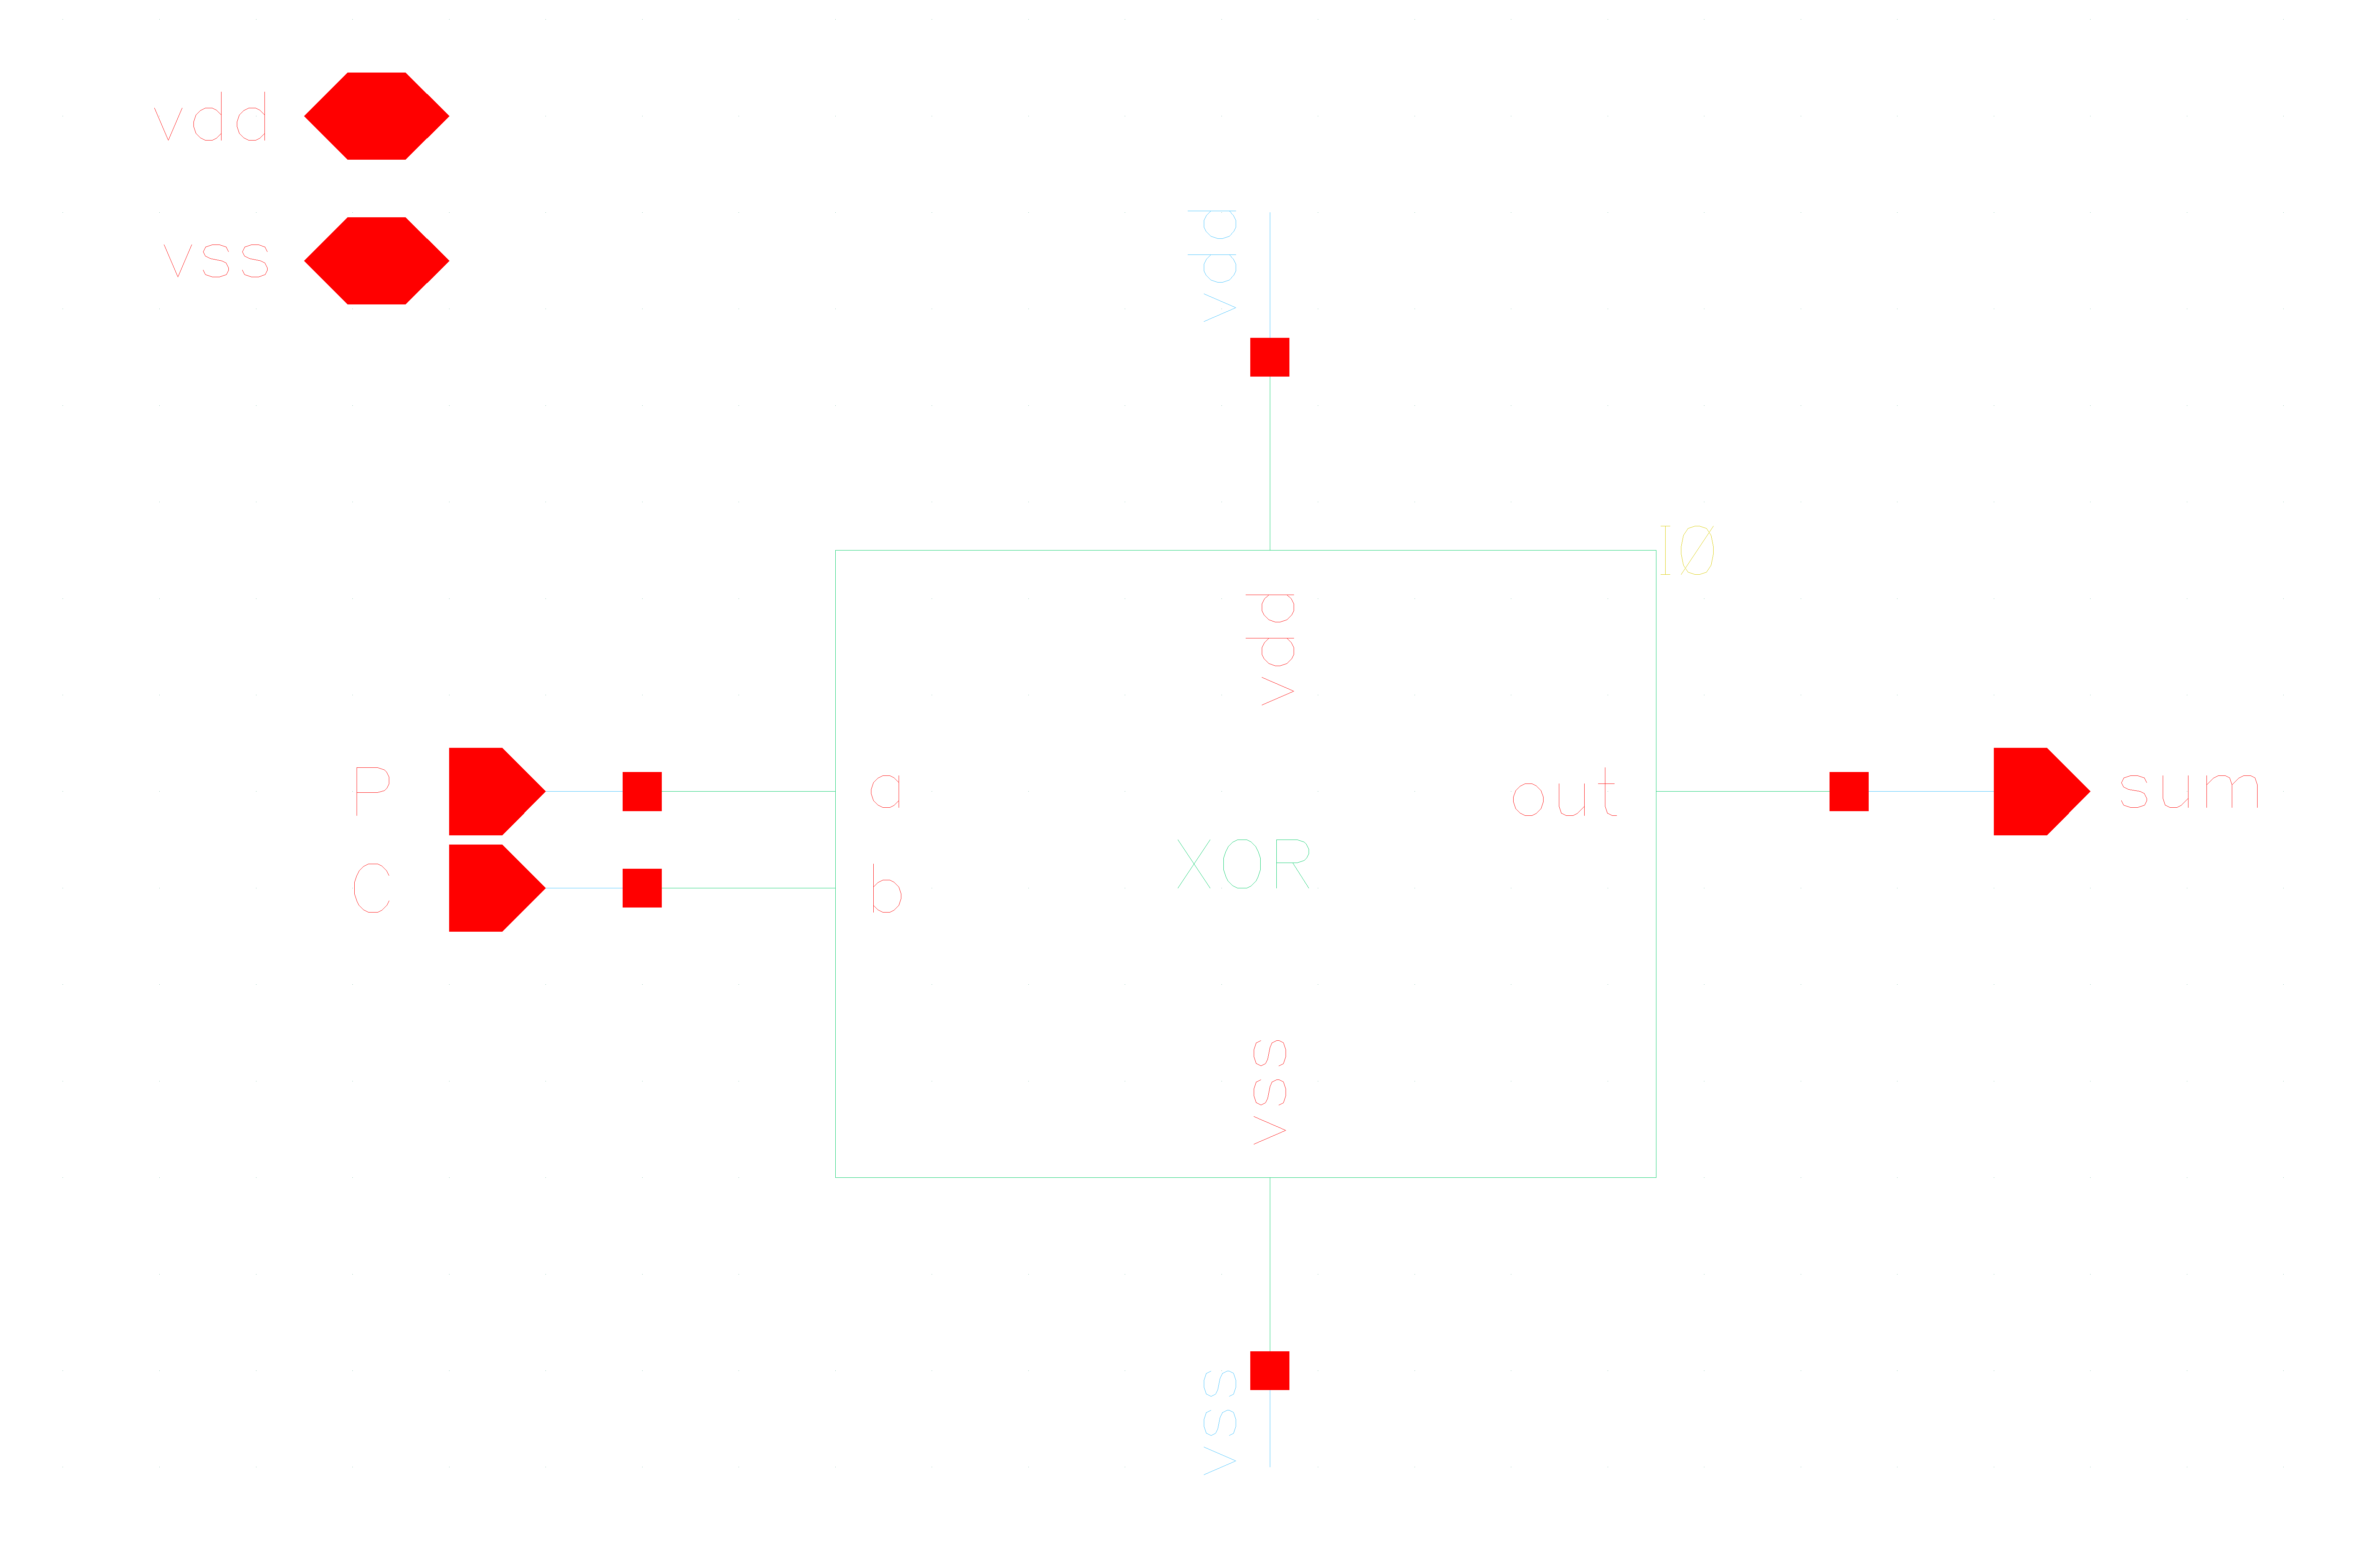
\includegraphics[clip,width=1.0\textwidth]{../figures/sum}
  \caption{Figure shows whats inside the sum block in the adder} \label{fig:sum}
\end{figure}
